\section{Tuesday, February 21st: Visual Design}
\subsection{Graphic Design}
\subsubsection{Communication}
\subsubsection{Interpretation}
\subsubsection{History}
Let's look at the start:\\
Materials are meant to be read and distributed, which means that you need to make sure texts are laid out in an understandable manner.

Terms such as upper case and lower case came from the separate cases used in printing presses -- \textit{terms which are still used today}.

\textbf{Main idea:} history influences the current state of design.

Churches or loyalties -- had lots of needs and wanted their words to be replicated. However after the 19th century, people have more disposable income so advertisements appear.

\subsubsection{Minimalism}
The London Underground is a great example of a simplistic yet `does its job' kind of logo which has withstood the test of time.

\subsubsection{Bauhaus Thinking}
Lots of Professors from the Bauhaus School of Art fled Nazi Germany and in going to the USA, etc they spread their thinking.

\myparagraph{Single axis of view}
A single vertical axis allows the user to read the text from top to bottom without confusion on where the next word(s) will be.

\myparagraph{Grid-based Design}
Every single element on the page is aligned to horizontal/vertical lines on an underlying grid.

Note that the grid does not have to be square or even axis-aligned, it just needs to be there to give structure.

\subsection{Visual Design}
\subsubsection{Corporate Identity}
IBM is a good example of a recognizable identity that is displayed on their posters as a brand mark.

\myparagraph{Logos}
This design of typefaces, size, color, etc is used even in Web Design -- think of the BBC news channel: their logo is recognizable and displayed on the top left of \href{https://www.bbc.com/}{https://www.bbc.com/}

\subsection{Product Design}
Product Design is about Form and Function.

\subsection{Streamlining}
This can be helpful but you should not take it too far.

\subsection{Form Follows Function}
\begin{shaded}
It is the pervading law of all things organic and inorganic,

Of all things physical and metaphysical,

Of all things human and all things super-human,

Of all true manifestations of the head,

Of the heart, of the soul,

That the life is recognizable in its expression,

\textbf{That form ever follows function.} This is the law.

- \textit{Louis Sullivan}
\end{shaded}

\subsection{Simplicity and Elegance}
\begin{shaded}
``Good artists borrow (from other artists), but great
artists steal!'' 

- \textit{Pablo Picasso}
\end{shaded}

\subsection{Simplicity}
Simple, minimalist, designs are often most effective. 

This is likely as there are less ways to interpret them (it has approachability, recognizability, and immediacy).

\subsection{Elegance}
The scrollbar is a good example of elegant design as it allows scrolling and indicates position in document.

\subsubsection{Reduction}
Only include essential elements.

\subsubsection{Regularization}
Use one set of shapes, colors, forms etc.

\subsubsection{Leverage}
Use elements in multiple roles.

\subsection{Unity}
One path to simplicity \& elegance is through unifying themes:\\
Forms, colors, components with like qualities.

Think of street signs.

\subsection{ Refinement}
Draw viewers’ attention to essential information.

Straighten subway lines to emphasize sequence of stops.

\begin{important}
Mistakes: Clutter \& Noise. Don't overdo it (especially with 3-D models on a 2-D screen).
\end{important}

\subsection{ Color}
\subsubsection{Color Spaces}
\myparagraph{Additive vs Subtractive}
Also known as RGB (red, green, blue) vs CMY (cyan, magenta, yellow).

These are used in Electronic Media and Printed Media respectively.

\subsubsection{Perceptual Organization}
There are 3-axes of color balance: Colorfulness, Hue, and Lightness. These parameterize our perception.

\subsubsection{Munsell Color Space}
Perceptually uniform book of painted chips

\begin{shaded}
Pro Tip:\\
Let Someone Else Pick For You
\end{shaded}

Some UI frameworks provide default themes... and color resources!

\subsection{ Gestalt Principles}
From Ware's 04 Paper:

\subsubsection{Figure/Ground}
Relative size.

\subsubsection{Proximity}
Introduce spacing/underlying grid.

Group related elements -- use size and typeface to allow scanning for groups.

\subsubsection{Similarity}
Can allow you to draw attention to one over the other $\in\{$rows, columns$\}$.

\subsubsection{Symmetry}
Bilateral symmetry gives strong sense of figure.

\subsubsection{Connectedness}
Connectedness overrules proximity, size, color shape.

\subsubsection{Continuity}
We prefer smooth not abrupt changes.

Connections are clearer with smooth contours.

\subsubsection{Closure}
\begin{center}
\begin{figure}[H]
    \centering
    
    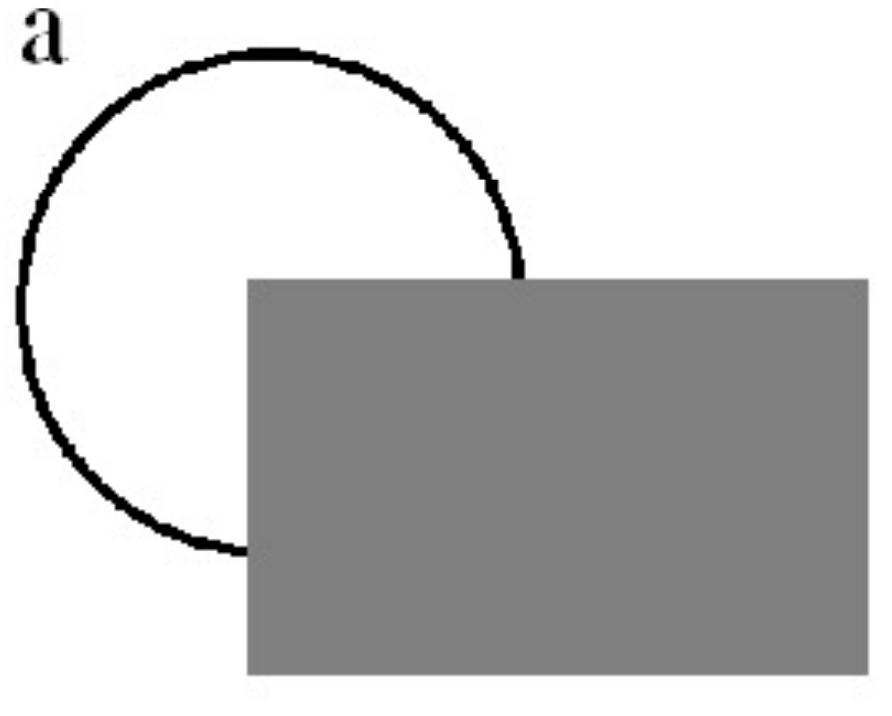
\includegraphics[scale=0.25]{lectures/wk6/img/a.png}
    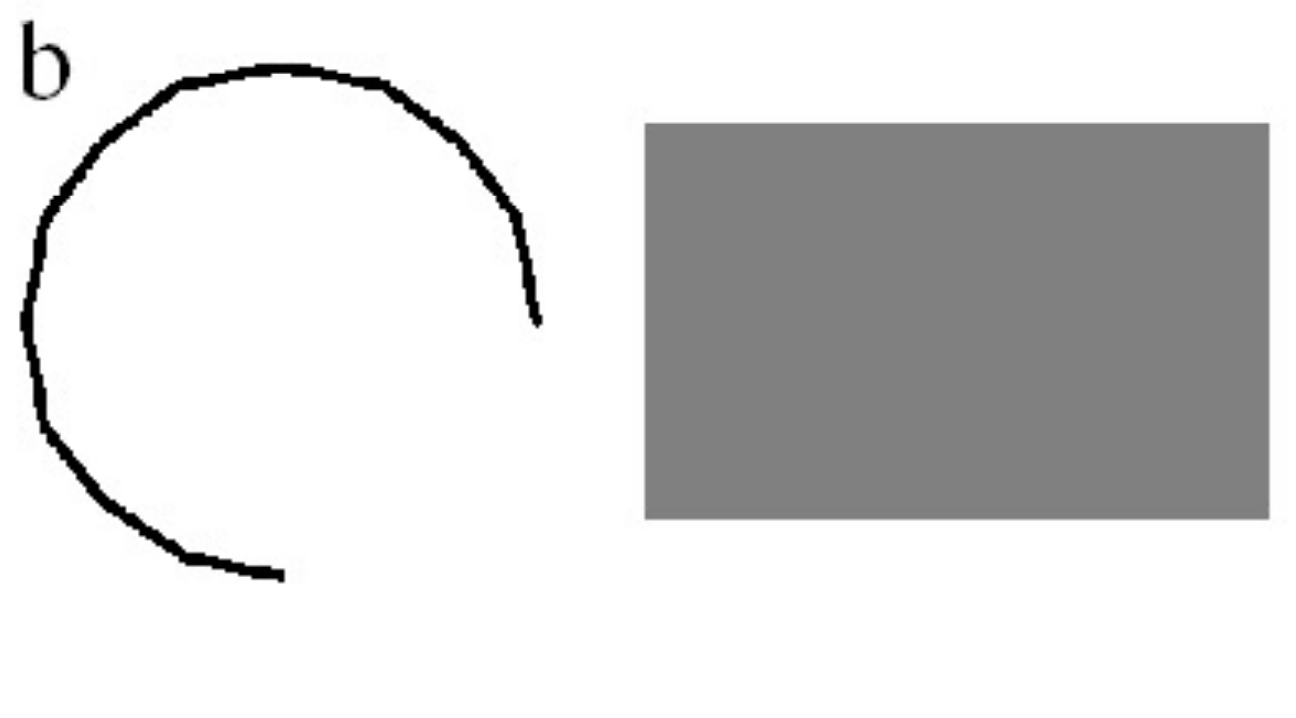
\includegraphics[scale=0.2]{lectures/wk6/img/b.png}
    
    \caption{We see a circle behind a rectangle, not a broken circle.}
\end{figure}
\end{center}

\subsubsection{Common Fate}
Dots moving together are grouped

\subsubsection{Transparency}

\subsection{ Fonts}
\subsubsection{Serif}
Flags/projections jetting off from the top of letters.

\subsubsection{Sans Serif}
Translates to ``Without Flags''

\subsubsection{Monospace}
A font where the space in between letters are fixed. The only use they have is for code/data/text where vertical alignment matters (i.e. Python code). 
\begin{important}
    You should not use this for long texts.
\end{important}